% Generated by Sphinx.
\documentclass[letterpaper,10pt,english]{manual}
\usepackage[utf8]{inputenc}
\usepackage[T1]{fontenc}
\usepackage{babel}
\usepackage{times}
\usepackage[Bjarne]{fncychap}
\usepackage{sphinx}


\title{Liz's Resume Documentation}
\date{July 21, 2009}
\release{1.0}
\author{liz}
\newcommand{\sphinxlogo}{}
\renewcommand{\releasename}{Release}
\makeindex
\makemodindex
\newcommand\PYGZat{@}
\newcommand\PYGZlb{[}
\newcommand\PYGZrb{]}
\newcommand\PYGaz[1]{\textcolor[rgb]{0.00,0.63,0.00}{#1}}
\newcommand\PYGax[1]{\textcolor[rgb]{0.84,0.33,0.22}{\textbf{#1}}}
\newcommand\PYGay[1]{\textcolor[rgb]{0.00,0.44,0.13}{\textbf{#1}}}
\newcommand\PYGar[1]{\textcolor[rgb]{0.73,0.38,0.84}{#1}}
\newcommand\PYGas[1]{\textcolor[rgb]{0.25,0.44,0.63}{\textit{#1}}}
\newcommand\PYGap[1]{\textcolor[rgb]{0.78,0.36,0.04}{#1}}
\newcommand\PYGaq[1]{\textcolor[rgb]{0.38,0.68,0.84}{#1}}
\newcommand\PYGav[1]{\textcolor[rgb]{0.00,0.44,0.13}{\textbf{#1}}}
\newcommand\PYGaw[1]{\textcolor[rgb]{0.13,0.50,0.31}{#1}}
\newcommand\PYGat[1]{\textcolor[rgb]{0.32,0.47,0.09}{#1}}
\newcommand\PYGau[1]{\textcolor[rgb]{0.13,0.50,0.31}{#1}}
\newcommand\PYGaj[1]{\textcolor[rgb]{0.00,0.44,0.13}{#1}}
\newcommand\PYGak[1]{\textcolor[rgb]{0.14,0.33,0.53}{#1}}
\newcommand\PYGah[1]{\textcolor[rgb]{0.00,0.13,0.44}{\textbf{#1}}}
\newcommand\PYGai[1]{\textcolor[rgb]{0.73,0.38,0.84}{#1}}
\newcommand\PYGan[1]{\textcolor[rgb]{0.00,0.44,0.13}{\textbf{#1}}}
\newcommand\PYGao[1]{\textcolor[rgb]{0.25,0.44,0.63}{\textbf{#1}}}
\newcommand\PYGal[1]{\colorbox[rgb]{1.00,0.94,0.94}{\textcolor[rgb]{0.25,0.50,0.56}{#1}}}
\newcommand\PYGam[1]{\textbf{#1}}
\newcommand\PYGab[1]{\textit{#1}}
\newcommand\PYGac[1]{\textcolor[rgb]{0.25,0.44,0.63}{#1}}
\newcommand\PYGaa[1]{\textcolor[rgb]{0.19,0.19,0.19}{#1}}
\newcommand\PYGaf[1]{\textcolor[rgb]{0.25,0.50,0.56}{\textit{#1}}}
\newcommand\PYGag[1]{\textcolor[rgb]{0.13,0.50,0.31}{#1}}
\newcommand\PYGad[1]{\textcolor[rgb]{0.25,0.44,0.63}{#1}}
\newcommand\PYGae[1]{\textcolor[rgb]{0.13,0.50,0.31}{#1}}
\newcommand\PYGaZ[1]{\textcolor[rgb]{0.02,0.16,0.45}{\textbf{#1}}}
\newcommand\PYGbf[1]{\textcolor[rgb]{0.40,0.40,0.40}{#1}}
\newcommand\PYGaX[1]{\textcolor[rgb]{0.00,0.44,0.13}{#1}}
\newcommand\PYGaY[1]{\textcolor[rgb]{0.25,0.44,0.63}{#1}}
\newcommand\PYGbc[1]{\textcolor[rgb]{0.00,0.44,0.13}{\textbf{#1}}}
\newcommand\PYGbb[1]{\textcolor[rgb]{0.13,0.50,0.31}{#1}}
\newcommand\PYGba[1]{\textcolor[rgb]{0.00,0.00,0.50}{\textbf{#1}}}
\newcommand\PYGaR[1]{\textcolor[rgb]{0.73,0.38,0.84}{#1}}
\newcommand\PYGaS[1]{\textcolor[rgb]{0.25,0.50,0.56}{\textit{#1}}}
\newcommand\PYGaP[1]{\textcolor[rgb]{0.25,0.44,0.63}{#1}}
\newcommand\PYGaQ[1]{\textcolor[rgb]{0.13,0.50,0.31}{#1}}
\newcommand\PYGaV[1]{\textcolor[rgb]{0.05,0.52,0.71}{\textbf{#1}}}
\newcommand\PYGaW[1]{\textcolor[rgb]{0.25,0.44,0.63}{#1}}
\newcommand\PYGaT[1]{\textcolor[rgb]{0.50,0.00,0.50}{\textbf{#1}}}
\newcommand\PYGaU[1]{\textcolor[rgb]{0.00,0.44,0.13}{#1}}
\newcommand\PYGaJ[1]{\textcolor[rgb]{0.25,0.44,0.63}{#1}}
\newcommand\PYGaK[1]{\textcolor[rgb]{0.02,0.16,0.49}{#1}}
\newcommand\PYGaH[1]{\fcolorbox[rgb]{1.00,0.00,0.00}{1,1,1}{#1}}
\newcommand\PYGaI[1]{\textcolor[rgb]{0.56,0.13,0.00}{#1}}
\newcommand\PYGaN[1]{\textcolor[rgb]{0.05,0.52,0.71}{\textbf{#1}}}
\newcommand\PYGaO[1]{\textcolor[rgb]{0.78,0.36,0.04}{\textbf{#1}}}
\newcommand\PYGaL[1]{\textcolor[rgb]{0.73,0.73,0.73}{#1}}
\newcommand\PYGaM[1]{\textcolor[rgb]{0.00,0.44,0.13}{#1}}
\newcommand\PYGaB[1]{\textcolor[rgb]{0.00,0.25,0.82}{#1}}
\newcommand\PYGaC[1]{\textcolor[rgb]{0.33,0.33,0.33}{\textbf{#1}}}
\newcommand\PYGaA[1]{\textcolor[rgb]{0.00,0.44,0.13}{#1}}
\newcommand\PYGaF[1]{\textcolor[rgb]{1.00,0.00,0.00}{#1}}
\newcommand\PYGaG[1]{\textcolor[rgb]{0.73,0.38,0.84}{#1}}
\newcommand\PYGaD[1]{\textcolor[rgb]{0.25,0.50,0.56}{\textit{#1}}}
\newcommand\PYGaE[1]{\textcolor[rgb]{0.63,0.00,0.00}{#1}}
\newcommand\PYGbg[1]{\textcolor[rgb]{0.44,0.63,0.82}{\textit{#1}}}
\newcommand\PYGbe[1]{\textcolor[rgb]{0.25,0.44,0.63}{#1}}
\newcommand\PYGbd[1]{\textcolor[rgb]{0.00,0.44,0.13}{\textbf{#1}}}
\newcommand\PYGbh[1]{\textcolor[rgb]{0.00,0.44,0.13}{\textbf{#1}}}
\begin{document}

\maketitle
\tableofcontents



hi\textasciitilde{} friends, I am liz, a stupid girl. I also have a nickname, Smelly Rabbit!
And more information is below:

\resetcurrentobjects


\chapter{关于Liz(About Liz)}


\section{我(I)}

我叫盛艳(非盛宴, 不然就是一桌好吃的\textasciicircum{}\%\$\#@*), 英文名lizzie(liz, for short). 我的英语很烂, 所以这文档是中西合壁\textasciitilde{}\textasciitilde{}

我是一名全职硕士研究生,,,可怜的已经念了20年的圣贤书, 终于终于终于...还有一年半毕业了! 在这20年中, 身心疲惫, 感觉自己活不了多久了:P,,,所以必得好好珍惜剩下的日子.


\section{喜欢的人和事(I like what?)}

I hate people who say much, do little things and 罗罗嗦嗦, 婆婆妈妈, 不爽快的人. 反之, 我喜欢和干脆, 利落, 直爽的人打交道,,,因为我本来就是心中藏不住东西的性格,,所以有啥秘密千万不要告诉你:P

I like watching classical movies and English songs. For example, the legend of fall, rain man, 阿甘正传..... 还有很多很多很多的英文歌, 最近喜欢一首歌叫做 \href{http://www.youtube.com/watch?v=py6vzbWJsCE}{We are one}, kelly sweet的.

另外, 欣赏好看的图片也是我一大乐趣, 因为小时候成绩特差, 经常被老师揪耳朵的那种, 不管那门功课几乎都是非常糟糕, 除了画画外, 所以从那时开始就定了个小小愿望, 就是长大后成为一名画家..包括初高中时临摹或自创的画有些很是不错的. 但可惜现在什么是退步了许多.


\section{我的朋友(My friends)}

从小到大, 当然有很多朋友, 有些是同学中要好的, 有些是一起玩着长大的, 还有一些是可以说说话的, 还有就是些比较特殊的, 剩下的人在我看来就是毫无交集的个体.

比较有个性的就是, 我定义了几个人物等级:
\begin{itemize}
\item {} 
完全陌生人(Complete strangers), 就是我不知道这世上有你, 你也不知道这世上有我的那些人;

\item {} 
陌生人(Strangers), 就是走在某条马路上, 看到周围好多好多陌生的面孔;

\item {} 
了解的人(Known people), 我知道的人, 可能不知道名字, 也可能知道, 但仅仅知道有这个人, 大概是干嘛的, 说实话并不想有深层次接触的人;

\item {} 
熟悉的人(Familiar with), 这里面就包括了一般同学, 老师, 邻居等等, 是个庞大的队伍; 说实话, 这也不是我所关心的人,,,因为一个字, 懒!

\item {} 
朋友(Friends), 普通朋友, 偶儿会互相帮助下的;

\item {} 
好朋友(Good friends), 饭会一起吃, 出去玩也会一起, 但是少了其中一人也不觉得缺了什么;

\item {} 
好好朋友(Good good friends), 一起长大, 或生病时会彼此关心的, 或有烦恼时发泄发泄的;

\item {} 
超级好朋友(Super good friends),,,,呵呵, 这个具有以上所有特点之外,,,最重要的一点就是, 他得经常被我欺负但不会生我气的人...这就是我的超级好朋友;

\item {} 
突然想到,,,还有一些,,算比较特殊(Special)的.

\end{itemize}

ok, break


\section{我的网上资源汇总(Resources)}
\begin{itemize}
\item {} 
主博客, \href{http://lizziesky.blogspot.com}{lizziesky}, 这是我最最早的博客;

\item {} 
我自己的网站, \href{http://liz.appspot.com}{lizsky}, 基于GAE制作的系列简单的不能再简单的网站;

\item {} 
\href{http://hi.baidu.com/lizziesky}{hi空间}, 百度hi上的空间, 不怎么用;

\item {} 
\href{http://www.douban.com/people/lizziesky/}{豆瓣};

\item {} 
\href{http://twitter.com/lizziesky}{twitter};

\item {} 
\href{http://www.flickr.com/photos/26211501@N07/}{flickr};

\item {} 
\href{http://lizziesky.haokanbu.com/}{好看簿};

\item {} 
\href{http://picasaweb.google.com/lizziesPicture}{picasa};

\item {} 
\href{http://www.diigo.com/dashboard/shengyan}{diigo};

\item {} 
\href{http://code.google.com/u/shengyan1985/}{code};

\item {} 
\href{https://github.com/lizzie}{github};

\item {} 
...

\end{itemize}


\section{杂七杂八(Mass)}

再写点其他的?

恩, 想到了,,,我是一个闲不住的人, 总是想找点事情做的那种, 所以就是劳累的命哪\textasciitilde{}
废话较少, 很随性格, 同时也是阴晴不定, 说话没头没尾, 记忆是选择性的, 思维比较混乱某些时候, 总体来讲, 就是一个小孩子, 外加上总会忍不住的傻笑.

总之, 缺点多多, 一言难尽!

over\textasciitilde{}

\resetcurrentobjects


\chapter{我的简历(Liz's Resume)}


\section{基本资料(Basic Info)}
\begin{itemize}
\item {} 
姓名: 盛艳

\item {} 
name: Yan Sheng

\item {} 
性别: 女

\item {} 
Sex: Female

\item {} 
出生年月: 1985年8月

\item {} 
Birthday: 1985, August

\item {} 
籍贯: 苏州

\item {} 
Origin: SuZhou

\item {} 
健康状况: 优秀

\item {} 
Health status: Excellent

\item {} 
毕业院校: \href{http://www.yzu.edu.cn}{扬州大学} 信息工程学院

\item {} 
Graduate institutions: Institute of Information Engineering, \href{http://www.yzu.edu.cn}{Yangzhou University}

\item {} 
专业/方向: 计算机应用技术/数据挖掘

\item {} 
Professional/Direction: Computer Application Technology/Data Mining

\item {} 
学历: 硕士/2010年七月毕业

\item {} 
Qualifications: Master/graduated in July 2010

\item {} 
手机: 13813147410

\item {} 
Mobile Phone: 13813147410

\item {} 
Email: \href{mailto:shengyan1985@gmail.com}{shengyan1985@gmail.com}

\item {} 
通信地址: 江苏省扬州大学信息工程学院400173\#

\item {} 
Communication Address: 400173\#, Institute of Information Engineering, Yangzhou University, JiangSu Province

\end{itemize}

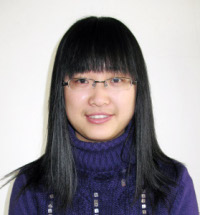
\includegraphics{mypic.jpg}


\section{工作意向(Job Objective)}
\begin{itemize}
\item {} 
软件开发工程师;

\item {} 
Software Development Engineer;

\item {} 
Web开发工程师;

\item {} 
Web Development Engineer;

\item {} 
维护?

\end{itemize}


\section{英语水平(English Ability)}
\begin{itemize}
\item {} 
于2004年获得CET-4证书;

\item {} 
In 2004, obtained CET-4 certificate;

\item {} 
具有扎实的英语应用能力及较强的计算机专业英文文献阅读及翻译水平, 并已发表多篇英文学术论文.

\item {} 
Have the good ability of English reading, writing, listening and speaking. Do well in reading or translating English literature of computer science and have published scholarly English papers.

\end{itemize}


\section{计算机能力/技能(Computer Ability and Skill)}
\begin{itemize}
\item {} 
精通 \href{http://www.python.org/}{Python}, 熟练使用基本Python库; C/C++相关基础知识扎实;

\item {} 
Proficient in \href{http://www.python.org/}{Python}, Familiar with the standard Python basis library;

\item {} 
熟悉Web应用开发; 熟练掌握Html, CSS, Javascript等Web技术, 并熟练使用 \href{http://jquery.com}{JQuery}, 有Ajax开发经验;

\item {} 
Familiar with the Web application development; Master Html, CSS, Javascript and other Web technologies, and  use \href{http://jquery.com}{JQuery} skilled, also have Ajax development experience;

\item {} 
掌握 \href{http://www.djangoproject.com/}{Django} 框架, 熟悉 \href{http://karrigell.sourceforge.net/}{Karrigell};

\item {} 
Become adroit at the \href{http://www.djangoproject.com/}{Django} Web development framework and know about \href{http://karrigell.sourceforge.net/}{Karrigell};

\item {} 
熟悉 \href{http://www.mysql.com}{MySQL}, \href{http://www.sqlite.org}{Sqlite} 等数据库使用;

\item {} 
Familiar with the use of \href{http://www.mysql.com}{MySQL}, \href{http://www.sqlite.org}{Sqlite} and other databases;

\item {} 
熟悉Linux/Unix类操作系统系统管理及维护;

\item {} 
Familiar with system management and maintenance of Linux/Unix-like operating system;

\item {} 
具有较扎实的算法理论知识;

\item {} 
Know many algorithms widely;

\item {} 
具有较强的理解问题, 分析问题能力, 对未知问题具有潜在的好奇心并不断通过各种方式找到解决方案;

\item {} 
Have better ability to understand and analyze problems and be very curious about the programming-related issues;

\item {} 
具有良好的编程风格, 对编码规范及文学化编程比较熟悉.

\item {} 
Have a good coding style and familiar with the coding rule and Literate Programming.

\end{itemize}


\section{教育经历(Education)}
\begin{itemize}
\item {} 
2007年9月\textasciitilde{}至今: 以优异成绩推荐免试于扬州大学信息工程学院, 攻读计算机应用技术专业/数据挖掘方向硕士学位, 现已完成前期基础课程的学习;

\item {} 
From September 2007 to now: studying in Institute of Information Engineering, Yangzhou University and doing some research about data mining;

\item {} 
2003年9月\textasciitilde{}2007年7月: 于扬州大学信息工程学院, 攻读计算机科学与技术(师范)专业学士学位, 完成本科阶段学习.

\item {} 
From September 2003 to July 2007: also learned lots of things in Institute of Information Engineering, Yangzhou University and obtained the bachelor's degree of Computer Science and Technology (Normal).

\end{itemize}


\section{主修课程(Majors)}
\begin{itemize}
\item {} \begin{description}
\item[本科阶段(2003年8月\textasciitilde{}2007年6月)]
\emph{基础课程:} 高等数学, 离散数学, 概率论与数理统计, 线性代数, PASCAL语言程序设计, C语言程序设计, C++程序设计, 汇编语言, 数据结构, 操作系统原理, 计算方法, 计算机通信, 编译原理, 数据库原理及应用, 面向对象技术, 计算机网络, 软件工程, 多媒体技术, 人工智能, 数字图像处理, 计算机组成原理, 微机原理, 单片机原理;

\end{description}

\item {} \begin{description}
\item[研究生阶段(2007年8月\textasciitilde{}2008年7月)]
\emph{基础课程:} 矩阵论, 数据仓库, 数据挖掘, 分布式数据库原理, 并行处理技术, 并行算法设计与分析, 计算机体系结构, 计算机网络技术, 最优化理论;

\emph{研究方向:} 数据挖掘, 概念格, 文本信息检索等. 熟悉多种数据挖掘算法及理论, 如: 经典Apriori, Decision Tree分类, 朴素贝叶斯分类, KNN分类, KMeans聚类, Rough Set Theory, Fuzzy Set Theory及形式概念分析中的Godin, Bordat算法等.

\end{description}

\end{itemize}


\section{发表论文(Publication)}
\begin{itemize}
\item {} 
SHENG Yan, LI Yun, TIAN Su-fang, LUAN Luan. A Rough Concept Lattice Model of Variable Precision. IEEE International Symposium on Intelligent Information Technology Application 2008 (IITA'08), Shanghai City, China;

\item {} 
Yun Li, Yan Sheng, Luan Luan, Lianglei Sun and Ling Chen. A Personalized Search Results Ranking Method Based on WordNet. 8th IEEE/ACIS International Conference on Computer and Information Science (ICIS 2009), June 1-3, 2009, Shanghai, China;

\item {} 
Li Yun, Sheng Yan, Luan Luan. A Text Classification Method with an Effective Feature Extraction based on Category Analysis.

\item {} 
盛艳, 李云, 李拓, 袁运浩. 一种基于概念格模型的本体合并方法. 2008全国开放式分布与并行计算学术年会(DPCS2008), 2008年10月25\textasciitilde{}27日;

\item {} 
盛艳, 李云, 李拓, 栾鸾. 基于概念格模型的本体映射. 第三届江苏计算机大会(Jiangsu Computer Conference 2008, JSCC 2008), 2008年11月14日\textasciitilde{}16日; 此论文被评为第三届江苏计算机大会"优秀论文";

\item {} 
栾鸾, 李云, 盛艳. 多关系频繁项集的并行获取. 2008全国开放式分布与并行计算学术年会(DPCS2008), 2008年10月25\textasciitilde{}27日;

\end{itemize}

上述论文可在 \href{http://github.com/lizzie/lizworkspace/tree/cb82ad8d84a1b1a12df80e3508e3629abf09ac83/paper}{这里} 找到.


\section{奖励/证书(Honors)}
\begin{itemize}
\item {} 
2003\textasciitilde{}2004学年获一等专业奖学金;

\item {} 
2003\textasciitilde{}2004学年被评为院"三好学生";

\item {} 
2004\textasciitilde{}2005学年获二等专业奖学金;

\item {} 
2004\textasciitilde{}2005学年被评为校"三好学生";

\item {} 
2005\textasciitilde{}2006学年获朱敬文奖学金;

\item {} 
2005\textasciitilde{}2006学年获校"优秀团员"称号;

\item {} 
2007学年获"优秀毕业生"称号;

\item {} 
2007\textasciitilde{}2008学年获研究生朱敬文奖学金.

\end{itemize}


\section{项目经历(Project Experience)}
\begin{itemize}
\item {} 
2007.12\textasciitilde{}2008.3 PR自动化工具
\begin{quote}

\emph{描述:} 由于学校的资料搜索系统涉及到很多脚本和程序文件数量很大, 为了使系统架构更加清晰, 也使开发维护人员更快更容易的理解整个流程, 设计并开发一个自动化脚本分析工具, 最大可能的呈现脚本, 程序, 配置文件之间的调用关系, 以便更好地理解整个系统.

\emph{Describe:} In order to understand the call relationships among files(scripts, program source files and configuration files) in the whole system quickly, we designed and developed a script analysis tools automatically. This tool also can search the keyword and print the search results in text or pictures.

\emph{职责:} Linux下Python实现后台脚本并使用命令行带参数解析模式, 解析输入文件, 将产生的文件之间的调用关系录入Mysql数据库; 前端使用Django开发, 实现查询文件并输出相关的信息(包括该文件调用的c, perl, python, shell脚本, conf配置文件等的图像或文本信息).

\emph{Duties:} The tools has two parts, one is to obtain the relations among lots of files and then save the relations to Mysql database in the backend; The other is a web interface developed by Django to retrieval the files which have certain keyword and related files(including c, perl, python, bash scripts, configuration files and text files).
\end{quote}

\item {} 
2007.9\textasciitilde{}2008.3 Galicia平台扩展
\begin{quote}

\emph{描述:} Galicia是个开源项目, 在此基础上实现形式概念分析中的一些概念格构造算法, 如Godin算法, Godin改进算法等, 分析算法的时间空间复杂度.

\emph{Describe:} Galicia is an open source project to implement concept lattice construction algorithms.

\emph{职责:} 在理解形式概念分析的基础上, 根据概念格自身特性, 掌握基本够格算法并实现, 之后图形显示结果格图, 以便更直观地得到概念格中概念及概念之间的继承关系.

\emph{Duties:} Improve the Godin algorithms to obtain better time and space complexity.
\end{quote}

\item {} 
2008.4\textasciitilde{}2008.11 Openbookproject开放图书计划
\begin{quote}

\emph{描述:} 中文Pythonic技术图书的翻译编写项目, 其工程网址在 \href{http://code.google.com/p/openbookproject/}{http://code.google.com/p/openbookproject}. 其中的LovelyPython是原创图书, 将Python以最易懂的方式介绍给读者, 可作为Python初学者急速入门图书.

\emph{Describe:} The project is about the translation or creatation of Chinese Pythonic books which is hold on \href{http://code.google.com/p/openbookproject/}{http://code.google.com/p/openbookproject}. LovelyPython is a original book which aimed to introduce the python to reader in the most understandable way and it can be a quick entry book for python beginners.

\emph{职责:} 参与LovelyPython图书整个创作过程, 具体有: PCS环境篇/语法篇/模块篇中大多数章节的编写, 实例故事练习题设计及解答及各种校对等. 由于此项目是基于google code, 所以非常熟悉分布式团队合作的整个过程.

\emph{Duties:} Took part in the whole creative process of LovelyPython. The detail: finished the most of chapters in the first three parts of PCS,  designed the exercises, many proofing works and so on. Since the project is based on the google code, I am very familiar with the whole process of distributed teamwork.
\end{quote}

\item {} 
2008.11\textasciitilde{}2009.01 禽流感病毒基因组生物信息学分析平台构建(Construction of Avian virus genome bioinformatics analysis platform)
\begin{quote}

\emph{描述:} 针对国际上各大生物信息中心提供的多个分析软件和基因/核酸数据库, 如BLAST检索系统(The Basic Local Alignment Search Tool, 一个基本的局部序列相似性比对搜索工具)及NCBI数据库(National Center for Biotechnology Information, 生物信息数据库中心), SMS2(The Sequence Manipulation Suite 2, 是用于分析较短的DNA和蛋白质序列的教学实验分析工具), Clustalx-2.0.10(用于进行DNA或蛋白质的多序列比对程序)等, 进行本地化生物信息学分析平台的构建, 并在此基础上进行功能扩展, 具体为禽流感病毒基因组数据库的选取, 定时更新及维护, 方便科研人员对禽流感病毒基因进行分析.

\emph{Describe:} Since major international Bioinformatics Center provide many anaysis software for gene and gene/nucleic acid database, such as, BLAST retrieval system(The Basic Local Alignment Search Tool) and NCBI database(National Center for Biotechnology Information), SMS2(The Sequence Manipulation Suite 2, for analyzing the shorter DNA or Protein sequence), Clustalx-2.0.10(Used for DNA or multiple protein sequence alignment tool), these analysis tools must be localized. Further more, some specail function need be extented, for instance, selecting the Avian virus genome from the complete database, then updating and other maintenance.

\emph{职责:} 完整搭建生物信息分析平台及其扩展. 主要有: 服务器基础环境安装及部署, 采用RedHat Enterprise Linux 4.0 AS作为服务器操作系统, 采用Apache2.2作为Web服务器及相关支持工具的安装. BLAST分析工具的本地化部署及相关数据库的安装, SMS2和Clustalx的安装部署, 并将三者整合起来. 其中, 基于Django0.96进行信息平台扩展并使用mod\_python部署到Apache上形成一整套完整的分析系统. 对系统扩展的工作主要有: 在所有基因数据库中提取禽流感病毒基因并构建二级数据库, 随着NCBI数据库的更新也随之更新并提供扩展检索功能.

\emph{Duties:} We installed RedHat Enterprise Linux 4.0 AS as server operating systems, Apache2.2 as Web server and other utilities. Then after localizing the BLAST, SMS2 and Clustalx, we integrated three systems to one complete system. The main extension is selecting the Avian virus genome to build a sub-database which updates with the NCBI database.
\end{quote}

\item {} 
2008.04\textasciitilde{}2009.01 各种使用Python编写的工具程序集(Many ToolSet )
\begin{quote}

\emph{描述:} 包含很多实用和非实用工具程序, 其项目网址为 \href{http://code.google.com/p/lizworkspace/}{http://code.google.com/p/lizworkspace/} . 主要有: Backup(备份两台机子上的监视文件以保持同步), streamdata(流数据上进行频繁项集的挖掘), perm(排列组合算法), mp3\_classify(将mp3歌曲根据歌手分类), powerset(产生集合的幂集), spider(本体实验中写的yahoo爬虫), search(分析google搜索结果用于个性化搜索实验), crontabanalysis(分析crontab文件), rmfilebaseondate(根据文件名上的日期删除文件), XMPP\_Jabber(基于XMPP/Jabber协议的机器人程序), godin(Godin算法, 序列, 模糊集, 粗糙集上的构格算法), FSproj(特征选择相关, 用于文本自动分类), Multi\_Relation(多关系上的贝叶斯分类).

\emph{Describe:} It includes many utilities which are in \href{http://code.google.com/p/lizworkspace/}{http://code.google.com/p/lizworkspace/}. Such as, Backup(Backup files which are in different computers to keep content consistent), streamdata(Mining the frequent item in stream data), perm(Permutation and combination algorithms), mp3\_classify(Classify the music based on singers), powerset(it produces one set's powerset quickly), spider(Yahoo spider used in my Ontology papers), search(Analyze the search result and user's web history from google used in Personalized Search), crontabanalysis(Analyze the crontab file to print information more human readable), rmfilebaseondate(remove the old files by date), XMPP\_Jabber(A simple robot  based on the XMPP/Jabber protocol), godin(Godin algorithm and other lattice-building algorithms used in Sequence, Fuzzy set and Rough set), FSproj(Feature Extraction to classify texts automatically), Multi\_Relation(Bayesian classifier in multi-relations data).
\end{quote}

\end{itemize}


\section{爱好/特长(Hobbies)}
\begin{itemize}
\item {} 
看电影, 听英文歌曲, 打羽毛球;

\item {} 
like classical movies, listening English songs and playing badminton;

\item {} 
喜欢玩各种图像处理软件和服务, 如PhotoShop, Illustrator, GIMP, Picasa等.

\item {} 
also be happy to play or use image processing software or services, such as PhotoShop, Illustrator, GIMP, Picasa and so on.

\end{itemize}


\section{自我评价(Self-evaluation)}
\begin{itemize}
\item {} 
责任心比较强, 能吃苦耐劳;

\item {} 
对人比较真诚, 有积极向上的乐观性格, 遇到困难不会轻易妥协;

\item {} 
容易和别人相处, 有比较强的团队精神;

\item {} 
I am a highly-motivated and reliable person with good health and pleasant personality. The main qualities required are preparedness to work hard, ability to learn with good analytical capability.

\end{itemize}


\section{谢谢:)(Thanks All)}

...


\renewcommand{\indexname}{Module Index}
\printmodindex
\renewcommand{\indexname}{Index}
\printindex
\end{document}
